\documentclass{article}

% Official NeurIPS 2026 position-track style.
\usepackage[position]{neurips_2026}

\usepackage[utf8]{inputenc}
\usepackage[T1]{fontenc}
\usepackage{hyperref}
\usepackage{url}
\usepackage{booktabs}
\usepackage{amsfonts}
\usepackage{nicefrac}
\usepackage{microtype}
\usepackage{xcolor}
\usepackage{graphicx}
\usepackage{subfigure}
\usepackage{amsmath}
\usepackage{amssymb}
\usepackage{mathtools}
\usepackage{amsthm}
\usepackage[capitalize,noabbrev]{cleveref}
\usepackage{textcomp}

\title{Brain-Conditioned Language Models Should Be Evaluated as Alignment Systems, Not Thought Decoders}

\author{%
  Anonymous Author(s) \\
  Anonymous Institution \\
  \texttt{anonymous@example.com}
}

\begin{document}
\maketitle

\begin{abstract}
This position paper argues that brain-conditioned language models should be evaluated as \emph{alignment systems}, not as direct ``thought decoders''.
Changing a language model's next-token distribution with an auxiliary vector is technically easy; showing that the change is grounded in stimulus-linked neural activity is much harder.
We argue that claims about brain-language generation require real neural supervision, temporal brain representations, and controls that distinguish aligned neural information from generic conditioning, dataset order, and language-model priors.
We support this position with preliminary diagnostic, negative, and corrective results: additive synthetic conditioning produces strong distributional deformation; shuffled and Gaussian controls can produce comparable deformation; prefix conditioning of a pretrained Qwen model fails to separate real from shuffled signals; and early T5--MEG experiments initially collapsed to language priors until temporal alignment, target leakage, and MEG scaling were corrected.
After these corrections, real post-word MEG windows produce a small but statistically reliable token-NLL improvement over both zeroed and shuffled brain controls on 50k MEG-MASC examples, while leaving top-1 predictions almost unchanged.
These results motivate a concrete protocol in which MEG-MASC provides real brain-language supervision, T5 cross-attends to temporal brain sequences, and The Virtual Brain is used only for temporal pretraining, augmentation, and perturbation analysis.
\end{abstract}

\section{Introduction}

\textbf{Position: brain-conditioned language models should be evaluated as controlled brain-language alignment systems, not as direct thought decoders; real stimulus-linked neural recordings must provide the supervision for brain-language claims, while neural simulators should be used for auxiliary temporal pretraining and perturbation analysis rather than as sentence-to-brain encoders.}

Language models are increasingly being connected to biological signals.
This direction is scientifically attractive because neural recordings may reveal information about perception, language comprehension, intention, memory, and internal state that is not present in text alone.
It is also practically attractive because language models provide strong priors for brain-computer interfaces and other systems that convert noisy neural measurements into communicative outputs.
At the same time, the combination of large language models and brain data creates a serious evaluation problem: a model may produce fluent text, or may change its token probabilities when a neural vector is injected, without using neural information in any meaningful sense.

The central claim of this paper is that brain-conditioned language modeling should be treated as an alignment problem.
The question is not simply whether a signal changes the output distribution.
Many signals can.
The question is whether a stimulus-linked neural signal changes the output distribution in a way that is predictive, temporally structured, robust to controls, and specific to the correct brain-text pairing.
Without this distinction, experiments risk confusing neural grounding with ordinary controllable generation.

This distinction is not only philosophical.
It directly affects how experiments should be designed.
If a simulated brain vector is paired with text by time index, and the vector was not generated as a response to that text, then successful conditioning does not show a brain-language relationship.
If the same projected vector is broadcast across every token position, then the model receives a global bias rather than a temporally structured brain signal.
If real and shuffled brain vectors produce similar likelihood gains, then the model may be using generic side information or regularization rather than aligned neural information.
If a model is evaluated only by Jensen-Shannon divergence from a zero-brain baseline, then any strong perturbation can look like success.

Our own preliminary work illustrates these risks.
We first trained brain-conditioned language models using simulated multi-region brain-like vectors paired with text contexts.
Those models produced measurable distributional deformation, and the deformation increased with the dimensionality of the auxiliary vector.
However, because the signals were simulated rather than stimulus-driven responses to the text, the results could not establish neural grounding.
We then tested prefix conditioning on a pretrained Qwen model.
The model optimized, and conditioning affected predictions, but controls showed that real and shuffled signals could behave almost identically.
Finally, in a first MEG-MASC/T5 cross-attention pilot, we found that naive training again produced misleading results: teacher-forced text context and incorrectly scaled MEG windows allowed the model to ignore brain input.
Only after removing decoder-side context leakage, using post-word MEG windows, and correcting signal normalization did REAL neural input begin to separate from ZERO and SHUF controls.
These results are not failures in the ordinary sense.
They are evidence that the field needs stricter standards for what counts as a brain-language result.

We propose a constructive alternative.
Real neural datasets such as MEG-MASC \citep{gwilliams2023megmasc} should provide the brain-language supervision.
Brain inputs should be temporal sequences, not static vectors.
Encoder-decoder models such as T5 \citep{raffel2020t5} should allow a text decoder to cross-attend to encoded brain dynamics.
The Virtual Brain (TVB) \citep{schirner2022brain} and related simulators should be used for temporal representation learning, augmentation, and controlled perturbation, not as ground-truth language supervision.
Evaluation should always include REAL/SHUF/ZERO controls, temporal perturbations, blocked splits, and separate reporting of distributional deformation and predictive utility.

\paragraph{Contributions.}
This paper contributes a position, a set of failure-driven arguments, and a concrete protocol.
First, we argue that distributional deformation is insufficient evidence for neural grounding.
Second, we show through preliminary results that simple additive conditioning and prefix conditioning can produce misleading effects without strong controls.
Third, we report a small but statistically reliable MEG-MASC pilot result after correcting target leakage and signal scale.
Fourth, we propose a real-data-centered architecture based on temporal brain encoding and decoder cross-attention.
Fifth, we define an evaluation protocol for separating genuine alignment from generic conditioning, shortcut learning, and language-model priors.

\section{From Brain Decoding to Brain-Language Alignment}

Neural decoding work has shown that brain activity can contain information about intended speech, handwriting, and language.
Intracortical systems have decoded attempted handwriting and speech at impressive rates \citep{makin2020handwriting,willett2021handwriting,moses2021neuroprosthesis,willett2023speechavatar}.
Non-invasive work has reconstructed semantic information from fMRI during continuous language comprehension \citep{tang2023semanticreconstruction}.
These results motivate brain-conditioned language modeling, but they also show why the evidentiary bar should be high.
Neural data are noisy, subject-specific, temporally structured, and strongly confounded by stimulus timing, task design, and preprocessing.

Brain-conditioned generation adds another complication: the language model itself is a powerful prior.
If a language model predicts a plausible continuation, it may be using the text context rather than the brain signal.
If an injected vector improves likelihood, it may be functioning as an auxiliary prompt, a dataset index, a subject/session code, or a source of regularization.
Therefore, the relevant scientific object is not text generation alone, but the alignment between neural dynamics and the changes induced in the language model.

We use three terms throughout the paper.
\emph{Deformation} refers to any change in the model's predictive distribution when a brain or brain-like signal is provided.
\emph{Utility} refers to whether that change improves prediction of the true continuation, usually measured by negative log-likelihood (NLL).
\emph{Alignment} refers to the stronger condition that utility depends on the correct stimulus-linked pairing between neural signal and language target.
Only the third notion supports a brain-language claim.

\begin{figure*}[t]
    \centering
    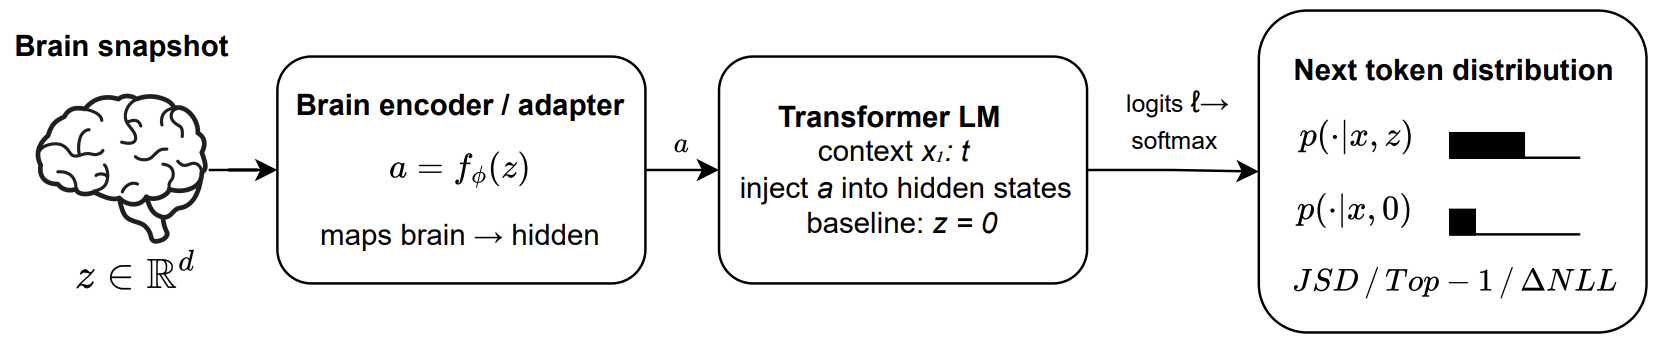
\includegraphics[width=\linewidth]{pipeline.png}
    \caption{
    Evaluation framing for brain-conditioned language models.
    The model may deform the next-token distribution under any nonzero auxiliary signal.
    A brain-language claim requires that REAL neural input improves predictive utility over both SHUF and ZERO controls, and that the model degrades under perturbations that destroy temporal or channel structure.
    }
    \label{fig:pipeline}
\end{figure*}

\section{Distributional Deformation Is Easy to Obtain}

Let $x_{1:t}$ be a text context, $z$ an auxiliary brain or brain-like signal, and
\[
p_\theta(\cdot \mid x_{1:t}, z)
\]
the next-token distribution of a conditioned language model.
A natural first diagnostic is to compare this distribution to a zero-signal baseline:
\[
\mathrm{JSD}\!\left(p_\theta(\cdot \mid x_{1:t}, z), p_\theta(\cdot \mid x_{1:t}, 0)\right).
\]
This measures how strongly the auxiliary signal changes the output distribution.
It does not measure whether the signal is useful, aligned, or neural.

This limitation is familiar from controllable generation.
Prefix tuning, prompt tuning, adapters, LoRA, and plug-and-play control all demonstrate that relatively small learned interventions can shift model behavior \citep{dathathri2020pplm,houlsby2019adapters,hu2021lora,li2021prefixtuning,lester2021prompttuning}.
Feature-wise modulation likewise shows that continuous side information can alter hidden representations \citep{perez2018film}.
Thus, showing that an auxiliary vector changes logits is not surprising.
For brain-language modeling, the minimum question must be stricter: does the correct neural signal improve prediction more than a matched but misaligned signal?

\section{Diagnostic Evidence From Preliminary Experiments}

Our preliminary experiments are useful because they expose exactly the evaluation traps that this position paper warns against.
We summarize them as diagnostic evidence rather than as final claims.

\subsection{Synthetic conditioning produces strong but ambiguous effects}

In a first set of experiments, we trained autoregressive language models conditioned on simulated multi-region brain-like vectors.
The model received a text context and a vector $z \in \mathbb{R}^d$.
The vector was projected into the model hidden size and injected into the Transformer.
Across dimensionalities, the auxiliary signal increasingly deformed the next-token distribution relative to a zero-signal baseline.

\begin{table}[t]
\centering
\caption{Legacy synthetic experiment: distributional deformation increases with simulated brain-vector dimensionality. This shows controllability of an auxiliary vector, not neural grounding.}
\label{tab:synthetic_dim}
\begin{tabular}{lccc}
\toprule
Dim. & JSD mean & JSD median & Top-1 agree \\
\midrule
68  & 0.0657 & 0.0511 & 0.681 \\
136 & 0.0736 & 0.0540 & 0.660 \\
272 & 0.0857 & 0.0718 & 0.620 \\
544 & 0.1359 & 0.1162 & 0.577 \\
\bottomrule
\end{tabular}
\end{table}

The result in Table~\ref{tab:synthetic_dim} is real but easy to overinterpret.
It shows that increasing the dimensionality of a side channel can increase the magnitude of distributional control.
It does not show that a real brain response is being used.
Because the vectors are simulated and not generated as stimulus-driven responses to the language input, the experiment cannot support claims about thought decoding or neural semantics.
At most, it establishes that a model can learn a controllable mapping from a continuous vector into token probabilities.

\subsection{Matched controls separate deformation from utility}

The synthetic setup also shows why deformation and utility must be reported separately.
For a 136-dimensional model, REAL, SHUF, and Gaussian-matched vectors produced nearly identical Jensen-Shannon divergence from the zero baseline, but only the nominal REAL condition improved NLL.

\begin{table}[t]
\centering
\caption{Legacy synthetic control result for a 136-D additive model. REAL, SHUF, and GAUSS produce comparable deformation, but only REAL improves NLL in this synthetic pairing.}
\label{tab:legacy_controls}
\begin{tabular}{lccc}
\toprule
Condition & JS mean & NLL mean & $\Delta$NLL vs.\ ZERO \\
\midrule
REAL  & 0.0737 & 2.417 & $-0.376$ \\
ZERO  & --     & 2.793 & $0.000$ \\
SHUF  & 0.0756 & 2.931 & $+0.138$ \\
GAUSS & 0.0739 & 2.932 & $+0.139$ \\
\bottomrule
\end{tabular}
\end{table}

This result is methodologically important.
If one reported only JSD, every nonzero condition would look similarly effective.
If one reported only NLL, the mechanism of change would remain opaque.
The combination reveals the relevant distinction: generic vectors can move the distribution, but useful movement requires the right pairing.
For real brain-language work, this same logic must be applied to real neural recordings and leakage-controlled splits.

\subsection{Pretrained decoder-only conditioning can hide misalignment}

We then moved from a small custom language model to a pretrained Qwen decoder with learned prefix tokens derived from the auxiliary vector.
This seemed architecturally more plausible because the pretrained model already supplies a fluent language prior, and the brain pathway only needs to steer it.
However, the controls exposed a different failure mode.

\begin{table*}[t]
\centering
\caption{Negative results from Qwen prefix conditioning on synthetic data. In the frozen-base setting, REAL and SHUF improve NLL almost identically. With the last two blocks unfrozen, both REAL and SHUF become worse than ZERO.}
\label{tab:qwen_negative}
\begin{tabular}{lcccc}
\toprule
Model setting & Condition & JS mean & NLL mean & $\Delta$NLL vs.\ ZERO \\
\midrule
Frozen base, prefix tokens & REAL & 0.0167 & 11.1460 & $-0.0861$ \\
Frozen base, prefix tokens & SHUF & 0.0142 & 11.1472 & $-0.0848$ \\
Frozen base, prefix tokens & ZERO & --     & 11.2321 & $0.0000$ \\
\midrule
Unfreeze last 2 blocks & REAL & 0.0080 & 11.6808 & $+0.0632$ \\
Unfreeze last 2 blocks & SHUF & 0.0079 & 11.6898 & $+0.0722$ \\
Unfreeze last 2 blocks & ZERO & --     & 11.6176 & $0.0000$ \\
\bottomrule
\end{tabular}
\end{table*}

In the frozen-base setting, REAL and SHUF improve NLL by almost the same amount.
This is not evidence for brain-language alignment.
It suggests that the prefix pathway may provide generic side information, alter calibration, or regularize decoding in a way that does not depend on correct pairing.
In the partially unfrozen setting, both REAL and SHUF worsen performance relative to ZERO, suggesting harmful overfitting or interference with the language prior.
These negative results motivate the position of this paper: stronger pretrained language models do not eliminate the need for stricter controls.
They may make those controls more important.

\subsection{A corrected MEG-MASC cross-attention pilot reveals a weak real signal}

We next implemented a real-data pilot using MEG-MASC recordings and a T5 encoder-decoder model.
The intended architecture was simple: a temporal brain encoder receives a MEG window with shape $T \times D$, projects it to the T5 hidden size, and the T5 decoder cross-attends to the resulting brain-time sequence while predicting target word tokens.
This experiment produced two instructive failures before producing a usable signal.

First, when the decoder was given the text context together with the target sequence under ordinary teacher forcing, REAL, SHUF, and ZERO conditions became indistinguishable.
The language model could predict from text context and token priors without using the brain stream.
Second, our initial MEG preprocessing used an additive $10^{-6}$ constant in the z-scoring denominator.
Because raw MEG values are stored in very small physical units, this constant overwhelmed the empirical channel standard deviations and collapsed the brain windows toward zero.
A diagnostic comparison found a mean absolute brain input of approximately $1.4 \times 10^{-7}$ and nearly identical encoder/logit outputs under REAL and ZERO inputs.
These are exactly the kinds of mundane implementation details that can create false negative or false positive conclusions in brain-language modeling.

We therefore rebuilt the pilot around three corrections.
We used post-word MEG windows ($0.0$--$0.6$ seconds after word onset), parsed word events directly from MEG-MASC timing metadata, removed decoder-side text-context leakage by training in a target-only decoder mode, and normalized each brain window before the temporal encoder.
We also restricted T5 adaptation to decoder cross-attention while keeping the language prior largely fixed.
Under this corrected setup, REAL MEG produced a small but statistically reliable NLL improvement over both ZERO and SHUF controls on 50k examples.

\begin{table*}[t]
\centering
\caption{Corrected MEG-MASC/T5 cross-attention pilot on 50k post-word examples. REAL uses the matched MEG window, ZERO removes the brain input, and SHUF permutes MEG windows across examples. Negative $\Delta$NLL means REAL is better. The effect is small and distributional: top-1 predictions are almost unchanged.}
\label{tab:meg_t5_pilot}
\begin{tabular}{lcccc}
\toprule
Condition & NLL mean & NLL median & $\Delta$NLL vs.\ REAL & Top-1 agreement vs.\ ZERO \\
\midrule
REAL & 6.8936 & 6.9045 & -- & -- \\
ZERO & 6.9048 & 6.9237 & $+0.0112$ & 0.9997 \\
SHUF & 6.9011 & 6.9119 & $+0.0075$ & 0.9997 \\
\bottomrule
\end{tabular}
\end{table*}

Paired analysis over examples gives $\Delta\mathrm{NLL}_{\mathrm{REAL-ZERO}}=-0.0112$ with 95\% CI $[-0.0126,-0.0098]$ and $\Delta\mathrm{NLL}_{\mathrm{REAL-SHUF}}=-0.0075$ with 95\% CI $[-0.0091,-0.0060]$.
The top-1 agreement between REAL and ZERO is $0.99968$, and between SHUF and ZERO is $0.99972$.
Thus, this is not open-vocabulary word decoding in any strong sense.
It is weak distributional brain sensitivity: the correct MEG signal nudges probability mass toward the target more than zeroed or mismatched MEG, but the model almost never changes its argmax prediction.

This result is valuable precisely because it is modest.
It supports our position better than an uncontrolled high-fluency demo would.
The failures show that language priors, teacher forcing, event parsing, and signal scaling can each erase or imitate brain effects.
The corrected pilot shows that once these issues are controlled, real MEG can produce a measurable but small alignment-specific improvement.
This is the kind of claim the field should make first: not that a model reads thoughts, but that a specific neural window produces a statistically reliable probability shift under strict controls.

\section{What Should Count as Brain-Language Supervision?}

For a brain-conditioned language model to make a neural claim, supervision should come from recordings obtained while subjects process language stimuli.
MEG-MASC provides one useful source of such supervision because it contains naturalistic story-listening MEG with rich linguistic annotations \citep{gwilliams2023megmasc}.
Other modalities, including fMRI, ECoG, and intracortical recordings, may support different versions of the same principle.
The key requirement is not the modality itself, but stimulus-linked alignment between neural activity and linguistic targets.

The basic training example should preserve temporal structure:
\[
(B_{t-\Delta:t}, x_{\leq t}, y_t),
\]
where $B_{t-\Delta:t}$ is a window of neural activity around a word or token, $x_{\leq t}$ is available linguistic context, and $y_t$ is the prediction target.
This formulation differs from treating the brain signal as a single vector.
It preserves the fact that language comprehension unfolds over time and that different brain channels and time bins may carry different information.

This also implies stricter data splitting.
Random example splits are dangerous because adjacent words in a story share neural context, stimulus context, and subject/session structure.
Evaluation should prefer leave-one-subject-out, leave-one-story-out, or blocked subject/story splits.
If random splits are used for early debugging, they should not be the basis of final claims.

\section{A Practical Architecture: Brain Encoder to T5 Cross-Attention}

We advocate a simple encoder-decoder architecture as a baseline for real-data brain-conditioned generation.
A temporal brain encoder maps a neural sequence into the hidden size of a pretrained encoder-decoder language model:
\[
H_B = \mathrm{BrainEncoder}(B_{1:T}) \in \mathbb{R}^{T \times d_{\mathrm{model}}}.
\]
The T5 encoder receives $H_B$ as continuous input embeddings, and the T5 decoder generates text while cross-attending to encoded brain states.

This architecture is not the only possible design, but it has several desirable properties.
It avoids broadcasting one static vector to every token position.
It gives the decoder a mechanism for selecting different brain time bins for different output tokens.
It permits attention analysis over brain time.
It also separates the temporal brain encoder from the language decoder, making it natural to pretrain the brain encoder on neural dynamics before supervised brain-to-text training.

The model should still be evaluated conservatively.
Cross-attention does not guarantee alignment.
Attention maps can be diffuse, unstable, or similar under REAL and SHUF conditions.
Nevertheless, cross-attention gives researchers an analyzable interface between brain time and generated text, which is preferable to a single opaque additive offset.

\section{The Proper Role of Neural Simulation}

TVB and related simulators are valuable, but they should not be treated as sentence-to-brain encoders.
Using simulated neural activity as if it were a ground-truth response to arbitrary text risks replacing a difficult empirical question with a synthetic shortcut.
If a simulator is not driven by the language stimulus, it cannot provide evidence that a language model has learned a brain-language relationship.

We propose three legitimate uses for TVB in this setting.
First, TVB can support self-supervised temporal pretraining of the brain encoder, using objectives such as masked reconstruction, next-step prediction, temporal order discrimination, or contrastive segment matching.
Second, it can provide augmentation and robustness tests over controlled time-series statistics.
Third, it can provide perturbation conditions: temporal shuffle, delay distortion, smoothing, region dropout, channel dropout, additive noise, or connectivity attenuation proxies.

Under this division of labor, real recordings provide the semantic and linguistic supervision.
TVB provides controlled dynamics and counterfactual interventions.
This preserves the usefulness of simulation without asking it to carry claims it cannot support.

\section{A Minimum Evaluation Protocol}

We propose the following minimum protocol for brain-conditioned language models.

\paragraph{Pairing controls.}
Every reported result should include REAL, SHUF, and ZERO.
REAL uses the correct neural signal paired with the target.
SHUF permutes neural signals across examples while preserving marginal statistics.
ZERO removes the neural signal.
A successful model should satisfy
\[
\mathrm{NLL}_{\mathrm{REAL}} < \mathrm{NLL}_{\mathrm{SHUF}}
\quad\text{and}\quad
\mathrm{NLL}_{\mathrm{REAL}} < \mathrm{NLL}_{\mathrm{ZERO}}.
\]
If REAL and SHUF are indistinguishable, the model has not demonstrated alignment.

\paragraph{Distributional and predictive metrics.}
Report deformation and utility separately.
Deformation metrics include Jensen-Shannon divergence, top-1 agreement, and logit-change magnitude.
Utility metrics include mean and median token NLL, $\Delta$NLL REAL-ZERO, and $\Delta$NLL REAL-SHUF.
The central warning is simple: deformation without utility is perturbation, not alignment.

\paragraph{Temporal perturbations.}
If a model claims to use temporal brain structure, it should degrade under temporal perturbations.
Useful perturbations include temporal shuffle, window reversal, smoothing, delay distortion, channel dropout, and region dropout.
The perturbations should be matched in marginal scale where possible, so that performance loss can be attributed to temporal or organizational disruption rather than trivial signal magnitude changes.

\paragraph{Blocked splits.}
Use subject-blocked and story-blocked splits when possible.
At minimum, report whether the split is random, subject-held-out, story-held-out, or both.
For naturalistic story data, adjacent windows are not independent.
This must be treated as an evaluation issue, not merely a data-loader detail.

\paragraph{Attention and subspace analysis.}
For cross-attention models, extract decoder cross-attention over brain time bins and compare REAL versus SHUF.
For logit-level analysis, inspect whether useful and harmful deformations occupy similar subspaces.
Our preliminary PCA analyses suggest that real and shuffled perturbations can share low-rank geometry; what matters is not only the rank or magnitude of deformation, but its direction relative to the correct token.

\section{Current Implementation}

We have implemented a first version of this protocol in a PyTorch and Hugging Face pipeline.
The pipeline preprocesses MEG-MASC recordings with MNE-Python, builds word-aligned sharded datasets, trains a T5 brain cross-attention model, evaluates REAL/SHUF/ZERO controls, and includes utilities for extracting decoder cross-attention.
The current working dataset contains 200k post-word MEG-aligned examples from preprocessed MEG-MASC recordings.
The current model uses a temporal brain encoder and a T5 decoder with target-only decoding, per-window brain normalization, and decoder cross-attention adaptation.

The first corrected evaluation produces the control pattern we require: REAL improves token NLL over both ZERO and SHUF on 50k examples.
The effect is small, however, and it barely changes top-1 predictions.
We therefore present it as preliminary evidence of weak distributional brain sensitivity, not as completed evidence of robust neural decoding or semantic grounding.
Rather, we present the implementation to make the position concrete.
The argument of this paper is not that a particular model has solved brain-conditioned generation.
The argument is that this is the kind of evidence a model should be required to produce before making a brain-language claim.

\section{Alternative Views and Objections}

\paragraph{Objection 1: synthetic proof-of-concept experiments are enough.}
Synthetic experiments are useful for debugging architecture and evaluation.
They can show whether a model can use an auxiliary vector.
They cannot show that the vector is a neural response to language.
For brain-language claims, the decisive evidence must involve real stimulus-linked recordings.

\paragraph{Objection 2: if a neural vector improves likelihood, then the model is using brain information.}
Likelihood improvement alone is not enough.
The vector may encode dataset order, subject identity, session artifacts, window position, or other shortcuts.
The improvement must survive SHUF, ZERO, blocked splits, and perturbations.

\paragraph{Objection 3: pretrained language models make neural alignment unnecessary.}
Pretrained language models are useful precisely because they supply strong linguistic priors.
But that strength also makes overclaiming easier.
A fluent output can be produced without relevant neural input.
The question is whether the neural signal changes the model's distribution in a pairing-specific and predictive way.

\paragraph{Objection 4: strict controls will make results smaller.}
They should.
The goal is not to maximize apparent effect size.
The goal is to identify the part of the effect that is actually supported by the neural signal.
For a field with obvious risks of mind-reading rhetoric, smaller controlled claims are preferable to larger ambiguous ones.

\section{Discussion}

Brain-conditioned language modeling sits between neuroscience, machine learning, and human-computer interaction.
This makes it exciting, but it also means that imprecise claims can travel quickly.
Terms such as ``thought decoding'' or ``brain-controlled language model'' can suggest a level of cognitive access that the evidence may not support.
The field should therefore distinguish clearly between three achievements: controlling a language model with a vector, improving prediction with a correctly paired neural signal, and explaining human cognitive representations.
Only the second and third require brain-language evidence, and the third requires substantially more than predictive performance.

Negative results should be treated as informative.
Our Qwen prefix experiments show that a stronger language prior can make controls more subtle rather than less necessary.
Our synthetic experiments show that deformation can be strong even when neural grounding is absent.
Our MEG-MASC pilot adds a complementary lesson: an apparently dead-flat REAL/ZERO/SHUF result can be caused by preprocessing scale collapse, while an apparently successful training loss can be caused by decoder-side language priors.
After correcting these issues, the remaining effect is real but small.
That smallness is itself informative: current cross-attention models may detect weak stimulus-linked structure in MEG, but they do not yet perform robust open-vocabulary word decoding.
These are not reasons to abandon brain-conditioned language modeling.
They are reasons to build the field around controls from the beginning.

The proposed protocol is intentionally conservative.
It may reject results that appear impressive under weaker evaluation.
That is a feature, not a defect.
Brain-language systems will eventually be used in high-stakes contexts, including assistive communication and clinical interfaces.
The community should require evidence that a model uses neural signals in the intended way before allowing output quality or distributional shift to stand in for neural grounding.

\section{Limitations}

This paper is a position paper, not a completed benchmark.
The MEG-MASC cross-attention experiments are preliminary and currently use random sampled examples rather than a full subject- or story-blocked benchmark.
The positive MEG-MASC result is a small token-NLL effect; it does not substantially change top-1 predictions and should not be interpreted as thought decoding.
The proposed protocol may be computationally expensive, especially for long-context encoder-decoder models.
MEG is noisy and nonstationary, and negative results under this protocol could reflect preprocessing choices, imperfect timing alignment, insufficient model capacity, or limited signal-to-noise ratio rather than absence of brain-language information.
Finally, token-level NLL is only one view of usefulness.
Future work should connect token-level alignment to sequence-level generation quality, communication efficiency, and human evaluation.

\section{Conclusion}

Brain-conditioned language models should be evaluated as alignment systems.
The core question is not whether an auxiliary vector can change a language model, but whether real stimulus-linked neural dynamics provide predictive information beyond matched controls.
This requires real neural supervision, temporal brain representations, architectures that can use temporal structure, and evaluations that separate deformation from useful aligned deformation.
Simulators such as TVB are valuable for temporal pretraining and perturbation analysis, but they should not replace real brain-language data.
Our preliminary MEG-MASC/T5 result illustrates both sides of the argument: naive configurations either ignored the brain stream or collapsed under preprocessing scale errors, while the corrected target-only post-word setup produced a small but reliable NLL advantage for REAL over ZERO and SHUF.
If the field adopts these standards, brain-conditioned generation can become a rigorous scientific and engineering program rather than a collection of impressive but ambiguous demonstrations.

\bibliographystyle{plainnat}
\bibliography{references}

\end{document}
